\subsection{Webes kliens megvalósítása}
Ez a fejezet a mobil kliens implementációjának részleteit mutatja be.
Nem minden funkció került megvalósításra, ezért csak azok a komponensek vannak részletezve amelyek a bemutatás során már működtek.

\subsubsection{Program felhasználói funkciói}
\begin{itemize}
    \item Regisztráció
    \item Bejelentkezés
    \item Kijelentkezés
    \item Oldalak közötti navigáció
    \item Művek, gyűjtemények böngészése, a kilistázó oldalon lapozás
    \item Művek, gyűjtemények megtekintése, fejezetek közötti és olvasása
    \item Művek megtekintése, fejezetek közötti és olvasása
    \item Bejelentkezett felhasználóknak további nézetek elérése
    \item Saját művek illetve gyűjtemények listájának megtekintése
\end{itemize}

\subsubsection{SPA Router}
A React applikációnkban a \texttt{React Router} (\url{https://reactrouter.com/}) \texttt{BrowserRouter}-e felelős az útvonalkezelésért.
Továbbá ez a csomag menedzseli a böngészési munkamenet (session) előzményeit és a ad számunkra navigációt elősegítő komponenseket (pl: Link, Navigate).
Az \texttt{SPA} (Single Page Application) azt jelenti, hogy csak egy webes dokumentumot tölt be a böngésző (ezesetben az \texttt{index.html}) és ennek a virtuális DOM-ját tölti fel dinamikusan.
Magukat az útvonalakat és a hozzá tartozó oldal-komponenseket a \texttt{AppRoutes} komponensünk definiálja.

\subsubsection{HTTP-kérések}
A HTTP kéréseket (GET, POST) a promise-alapú \texttt{Axios} (\url{https://axios-http.com/}) JavaScript könyvtárral intézzük.
A backenddel való kommunnikációhoz szükséges konfigurációk az \texttt{api/axios.jsx}-ben vannak

\subsubsection{Context Provider}
Az authentikáció után állapotaként a felhasználóhoz tartozó egyes adatokat (illetve az CSRF elleni tokent) a \texttt{ContextProvider} komponens szolgáltatja a struktúrában a gyerekeinek.
Azok az \texttt{useAuthContext} hook-ot használva tudnak hozzáférni az adatokhoz, megelőzve a sok props leadogatást a komponenseknek.

\subsubsection{Navigálás a weboldalon}
Navigálásban főként a felső sávban elhelyezkedő menük és gombok segítenek.
\begin{itemize}
    \item \textbf{/} (átirányít a /works-re)
    \item \textbf{/works}
    \item \textbf{/collections}
    \item \textbf{/reader}
    \begin{itemize}
        \item \textbf{\dots/[workID]}
    \end{itemize}
    \item \textbf{/collection}
    \begin{itemize}
        \item \textbf{\dots/[collectionID]}
    \end{itemize}
    \item \textbf{/login} (visszairányít, ha a felhasználó már be van jelentkezve)
    \item \textbf{/register} (visszairányít, ha a felhasználó már be van jelentkezve)
    \item \textbf{/profile} (átirányít a /login-ra, ha a felhasználó nincs bejelentkezve)
    \item /\textbf{account} (átirányít a /login-ra, ha a felhasználó nincs bejelentkezve)
    \item \textbf{/editor} (mű szerkesztő, még nem kommunikál)
\end{itemize}

\subsubsection{Webes felhasználói felület}
A weboldal felülete a \texttt{React MUI} (félkész és konfigurálható) komponenseivel van felépítve.
Ez a csomag azért lett választva, hogy a dizájn a mobilossal valamilyen szinten megegyezzen.
Ahogyan már az előbbiekben említettük, a SPA egyetlen dokumentumát tölti fel az alkalmazás;
emiatt a navigáció zökkenésmentesnek hat.

A weboldal látogatásakor tipikusan a Művek böngészése oldalra kerül a felhasználó.

\begin{figure}[H]
    \centering
    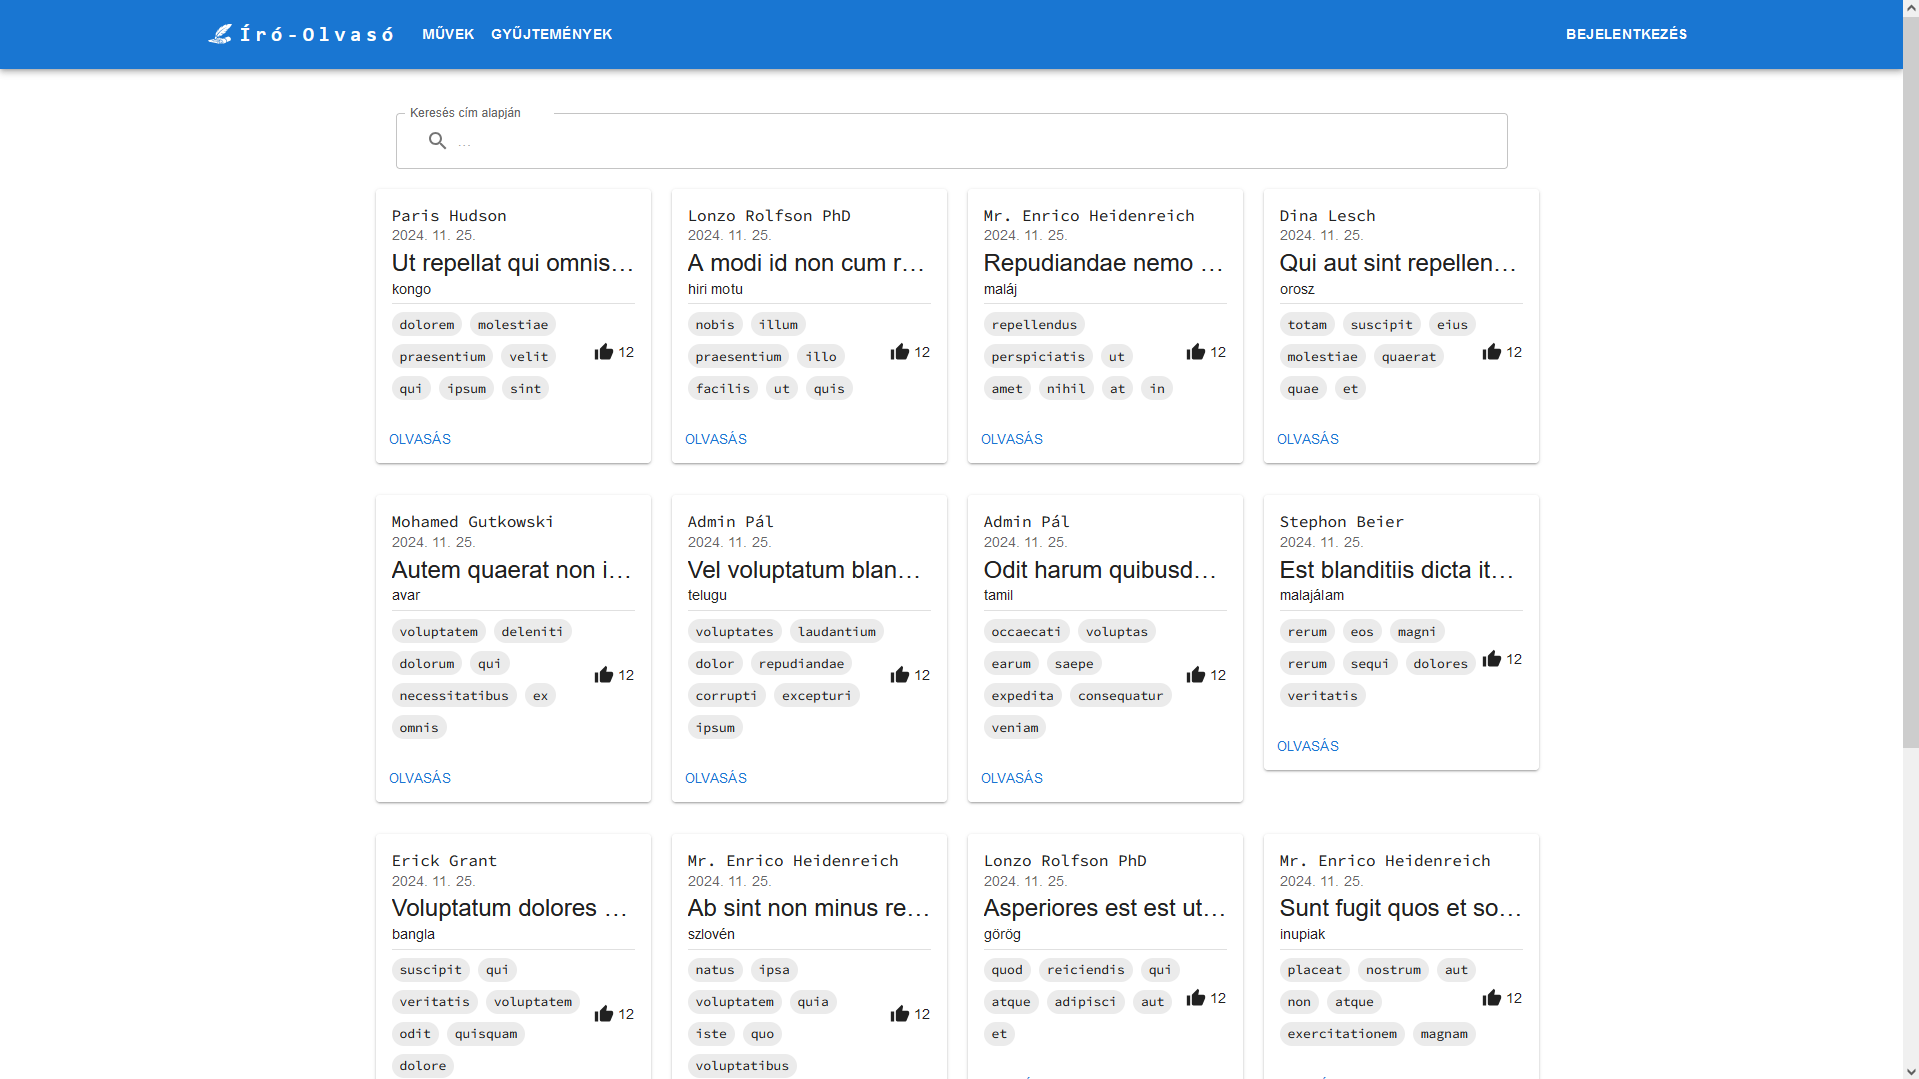
\includegraphics[scale=0.3]{./figures/works-page.png}
    \caption{/works Művek oldal}
    \label{fig:works-page}
\end{figure}

A felső navigációs sávban láthatja a másik nem bejelentkezett látogatók
számára is elérhető Gyűjtemények oldalt, továbbá a Bejelentkezés gombot.
Kisebb képernyőmérettel vagy ablakmérettel az oldal tartalma is alkalmazkodik.
Ilyenkor a navigációs sáv opció egy lenyíló menüben érhetők el.

\begin{figure}[H]
    \centering
    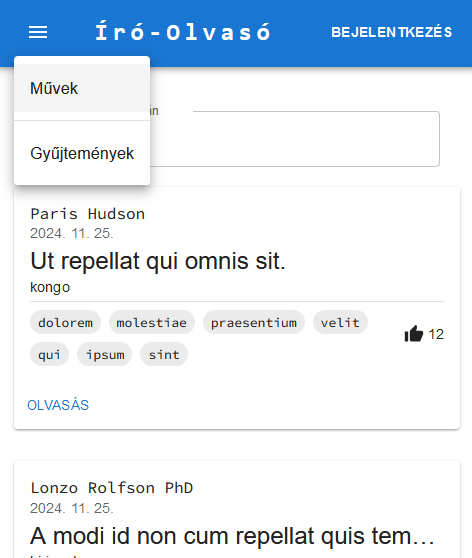
\includegraphics[scale=0.5]{./figures/navbar-small.png}
    \caption{Művek oldal kisebb méretben}
    \label{fig:navbar-small}
\end{figure}

Az oldal legalján lehet lapozni, mivel nem minden kártya fér ki egy oldalra (jelenleg 15 kártya / oldal van beállítva).
A szélső gombok sorrendben az első és utolsó oldalra lapoznak. A Gyűjtemények oldal hasonló kártyákkal és lapozással van ellátva.

\begin{figure}[H]
    \centering
    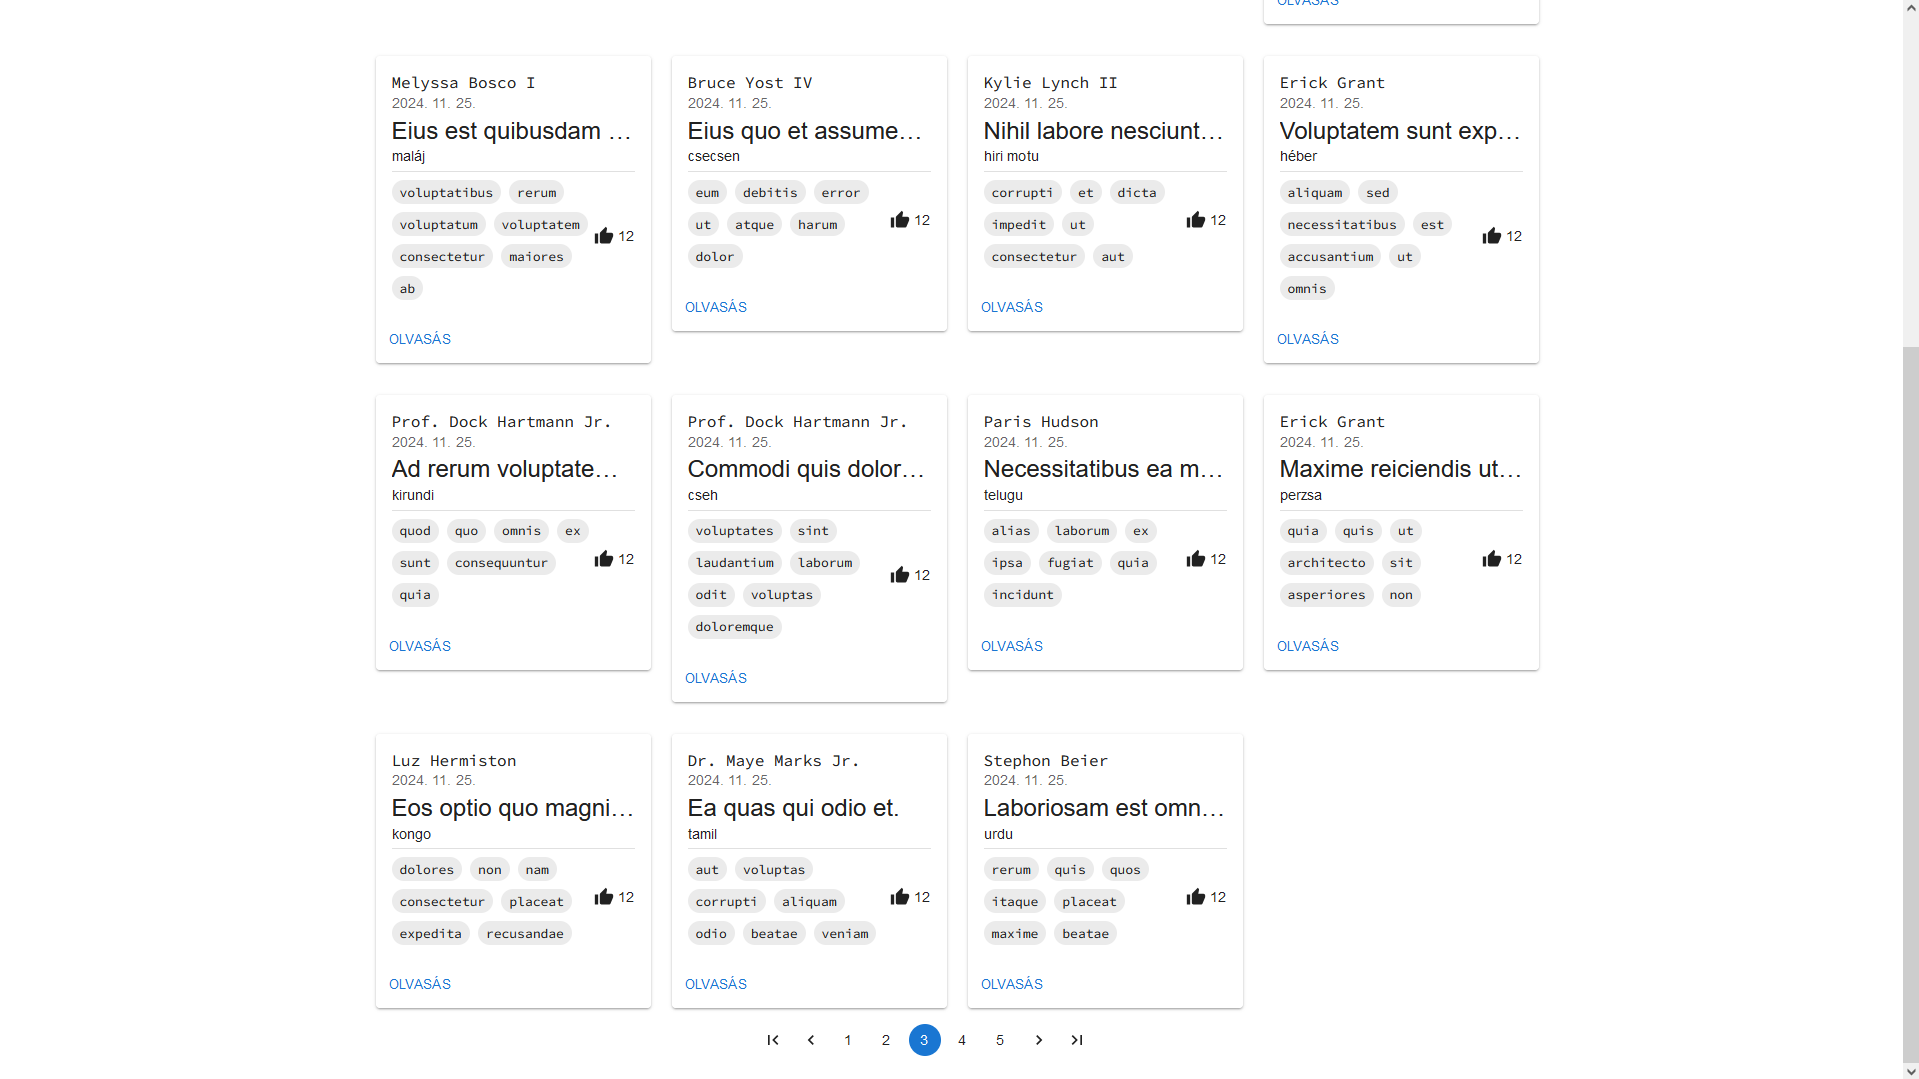
\includegraphics[scale=0.3]{./figures/works-pagination.png}
    \caption{Művek oldal lapozása}
    \label{fig:works-pagination}
\end{figure}

Ha egy Gyűjteményt a kártyáján megjelenő gombbal megnyitunk, átvisz minket a /collection/[ID] útvonalra.
Itt a gyűjteménybe szedett művek listáját kapjuk meg, továbbá láthatjuk, hogy mennyi kedvelést illetve milyen hozzászólásokat kapott.

\begin{figure}[H]
    \centering
    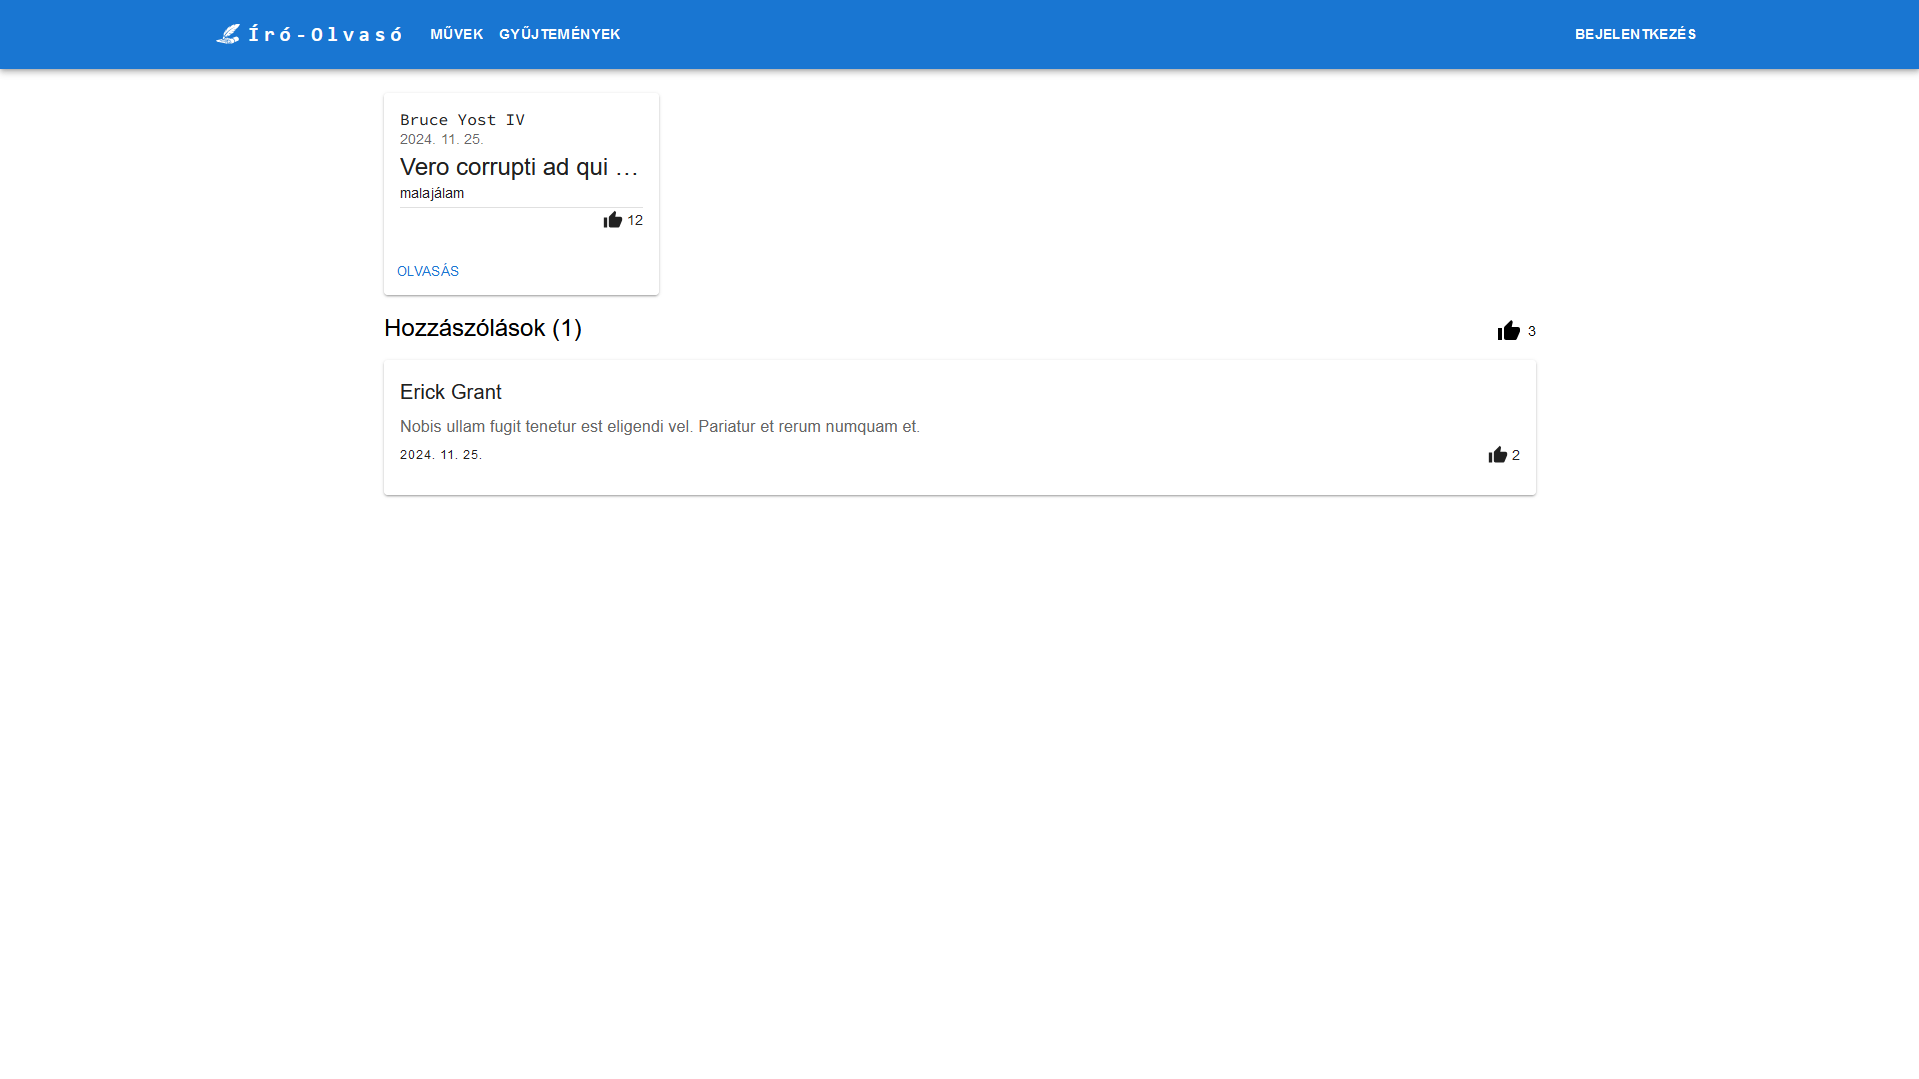
\includegraphics[scale=0.3]{./figures/collection-page.png}
    \caption{Gyűjtemény megtekintése}
    \label{fig:collection-page}
\end{figure}

A gyűjteményben lévő műveket is meg lehet nyitni, hogy elolvassuk.

